\documentclass[12pt, titlepage]{article}
\usepackage[bottom = 3cm, top = 3cm, left = 3cm, right = 3cm]{geometry}
\usepackage[english]{babel}
\usepackage[utf8]{inputenc}
\usepackage[table]{xcolor}
\usepackage{graphicx, booktabs, tikz, csquotes, subcaption, enumitem, dcolumn, pdfpages}
\usepackage[font=normalsize]{caption}%,labelfont=bf

\renewcommand*\rmdefault{ppl}

\usepackage{setspace}
\setstretch{1.5}

\usepackage[]{titlesec}
    \titleformat*{\section}{\large\bf}
    \titleformat*{\subsection}{\normalsize\it}

% Bibliography
% \usepackage[natbibapa]{apacite}
\usepackage[round]{natbib}
% \renewcommand{\bibliographytypesize}{\normalsize}
\setlength{\bibsep}{5pt}

\usepackage[colorlinks = TRUE, allcolors = blue]{hyperref}

\widowpenalty=10000
\clubpenalty=10000

\title{\Large Online Appendix for:\\Do TJ policies cause backlash?\\Evidence from street name changes in Spain}
\author{}
% \author{Francisco Villamil\thanks{Juan March Institute--Carlos III University of Madrid, francisco.villamil@uc3m.es} \and Laia Balcells\thanks{Georgetown University, lb1127@georgetown.edu}}
\date{\today}

\renewcommand{\thesection}{A\arabic{section}}

\begin{document}

\maketitle

\tableofcontents
% \listoffigures
% \listoftables


\clearpage
\section{Francoist street names}\label{franc_names_list}

We considered as Francoist the following street names. The starting point was the list published by the Madrid City Council in 2017, where they proposed a list of 52 street names to be removed, following a report by the Historical Memory Commission.\footnote{The full list and the reasons for the choice of each street name is available online at https://bit.ly/37cLGgk (accessed 26/11/2020).}
This list was expanded, manually selecting from the street names most commonly changed.
Indeed, among all the changes between 2001 and 2020, the five most commonly removed street names were all key Francoist figures: `Jose Antonio,' `Calvo Sotelo,' `General Mola,' `Generalísimo,' and `General Franco.' The full list:

\begin{quote}
  18 de Julio; Alcalde Conde de Mayalde; Alcazar; Alcazar de Toledo; Alferez Provisional; Almirante Francisco Moreno; Angel del Alcazar; Arco de la Victoria; Arriba Espana; Aunos; Batalla de Belchite; Batalla del Ebro; Caidos; Caidos (de Los); Caidos (los); Caidos de la Division Azul; Caidos Por la Patria; Calvo Sotelo; Calvo Sotelo (de); Capita Cortes; Capitan Cortes; Capitan Cortes (del); Capitan Haya; Capitan Luna; Carlos Pinilla; Carlos Ruiz; Carrero Blanco; Caudillo; Caudillo (del); Cerro de Garabitas; Cirilo Martin Martin; Comandante Franco; Comandante Franco; Comandante Zorita; Conde Vallellano; Crucero Baleares; Defensores del Alcazar; Defensores del Alcazar; Dieciocho de Julio; Diego Salas Pombo; Division Azul; Doctor Vallejo-Nagera; Eduardo Aunos; Ejercito Espanol; El Algabeno; Emilio Jimenez Millas; Falange Espanola; Federico Mayo; Federico Servet; Fernandez Ladreda; Francisco Franco; Franco; Garcia Morato; General; General Aranda; General Asensio Cabanillas; General Cabanellas; General Cabanellas; General Davila; General Fanjul; General Franco; General Garcia de la Herranz; General Garcia Escamez; General Kirkpatrick; General Millan Astray; General Mola; General Mola (del); General Moscardo; General Munoz Grandes; General Orgaz; General Primo de Rivera; General Queipo de Llano; General Rodrigo; General Romero Basart; General Sagardia Ramos; General Saliquet; General Sanjurjo; General Varela; General Yague; Generalisimo; Generalisimo (del); Generalisimo Franco; Gobernador Carlos Ruiz; Hermanos Falco y Alvarez de Toledo; Hermanos Garcia Noblejas; Heroes del Alcazar; Jose Antonio; Jose Antonio (de); Jose Antonio Giron; Jose Antonio Giron; Jose Antonio Primo de Rivera; Jose Luis de Arrese; Jose Maria Peman; Juan Pujol; Juan Vigon; Lepanto; Los Martires; Manuel Sarrion; Martires; Martires (los); Matias Montero; Millan Astray; Munoz Grandes; Onesimo Redondo; Pilar Primo de Rivera; Primero de Octubre; Primo de Rivera; Puerto de los Leones; Queipo de Llano; Ramiro Ledesma; Ramon Franco; Ruiz de Alda; Salas Pombo; Veintiocho de Marzo

\end{quote}

\clearpage
\section{DiD sample and treatment strength}

Figure~\ref{fig:trt_strength_st2016} shows the treatment strength (i.e. the number of Francoist name removals) depending on the number of streets with Francoist names in June 2016. Because of scale problems, the city of Madrid was removed from the graph, even though it follows a similar pattern: Madrid had 60 streets with Francoist names in mid 2016, and removed 52 of those during the period.
The graph shows that most streets had very few streets in 2016 and removed those (usually 1 or 2), while a small subset had more streets and removed either all or part of them.

Figure~\ref{fig:trt_remaining} shows the distribution of remaining streets with Francoist names on January 1st, 2019, among those municipalities that were classified as treated in the analyses.
Most municipalities that were treated between mid 2016 and late 2018 removed all their streets with Francoist names, and only a small minority retained a small number of Francoist streets (mostly one or two).

In many cases, differences in treatment strength---and the fact that there were remaining Francoist streets names after this period---is due to the fact that the list of Francoist names we use (list in previous section \ref{franc_names_list}) is very comprehensive: many municipalities likely removed the most famous and relevant Francoist names, which arguably were the ones most likely to produce some kind of effect on local political preferences.

\begin{figure*}[htb!]
\centering

  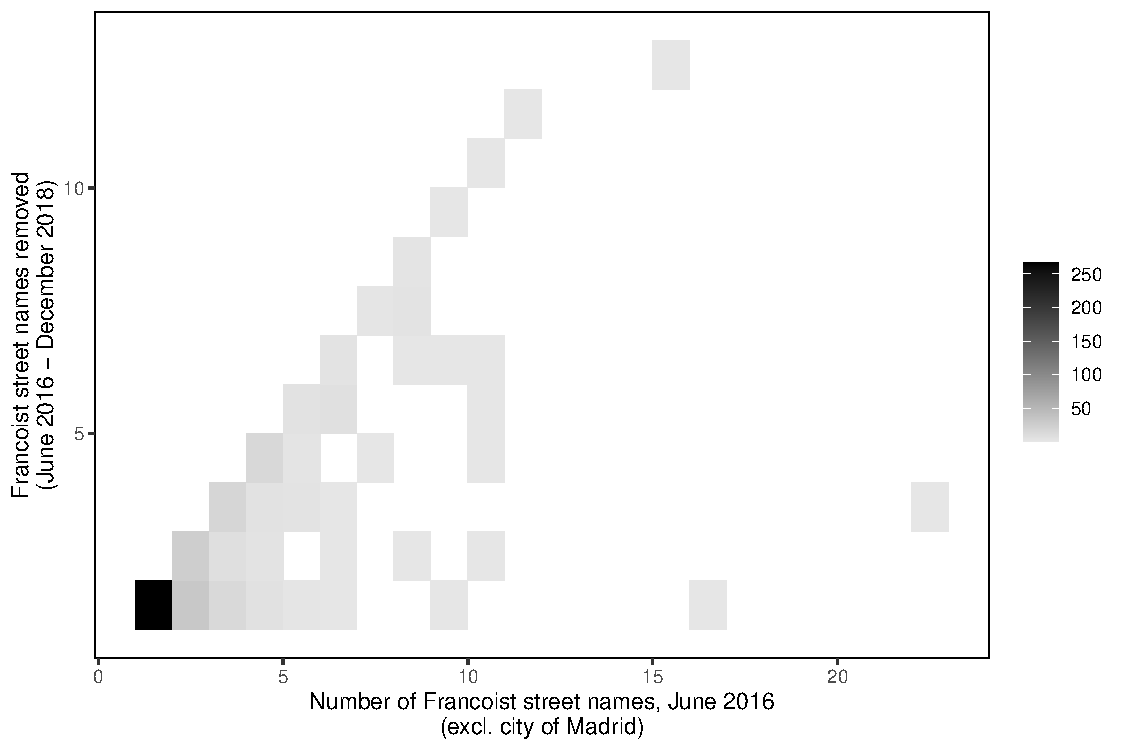
\includegraphics[width = 0.75\textwidth]{img/trt_strength_st2016}

  \caption{Treatment strength among the treated}\label{fig:trt_strength_st2016}

\end{figure*}

\begin{figure*}[htb!]
\centering

  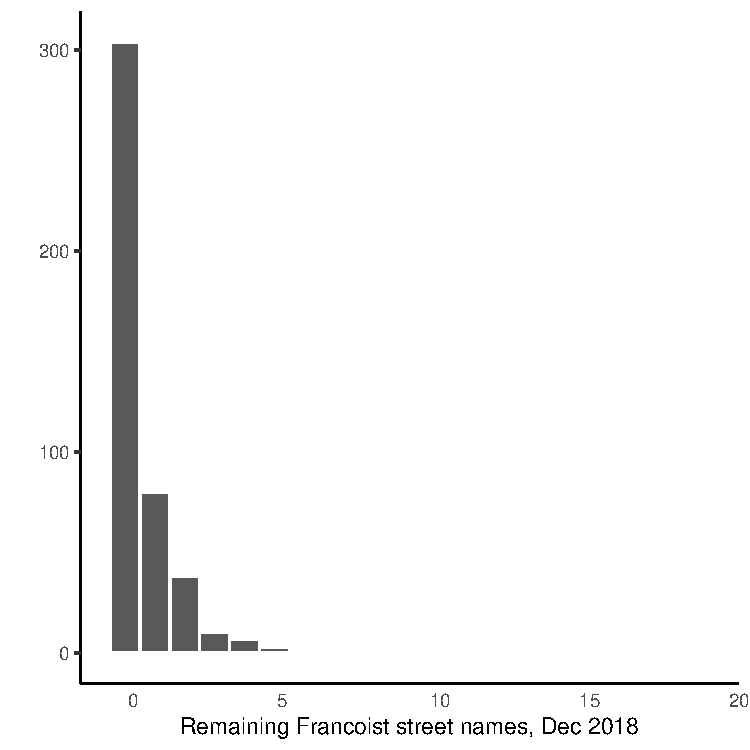
\includegraphics[width = 0.6\textwidth]{img/trt_remaining}

  \caption{Remaining Francoist streets on treated municipalities `after treatment'}\label{fig:trt_remaining}

\end{figure*}


\clearpage
\section{Descriptives on Francoist street name removals}

Figure~\ref{fig:changes_by_prov} shows the number of Francoist street name removals by province in three different time periods: 2001--2020, 2011--2016, and 2016--2018.
Figure~\ref{fig:fs_by_prov} shows the share of Francoist street by province at three different points in time: June 2001, January 2010, and June 2016.
A quick look shows that provinces that removed more Francoist streets during the whole available period are similar to those that removed more Francoist names between 2016 and 2019, which are also provinces that had a higher share of Francoist streets in 2001.
These are mostly provinces in central Spain, where Francoist streets were not removed earlier on either because of inertia or ideological opposition, as discussed in the main text.

\begin{figure*}[htb!]
\centering

  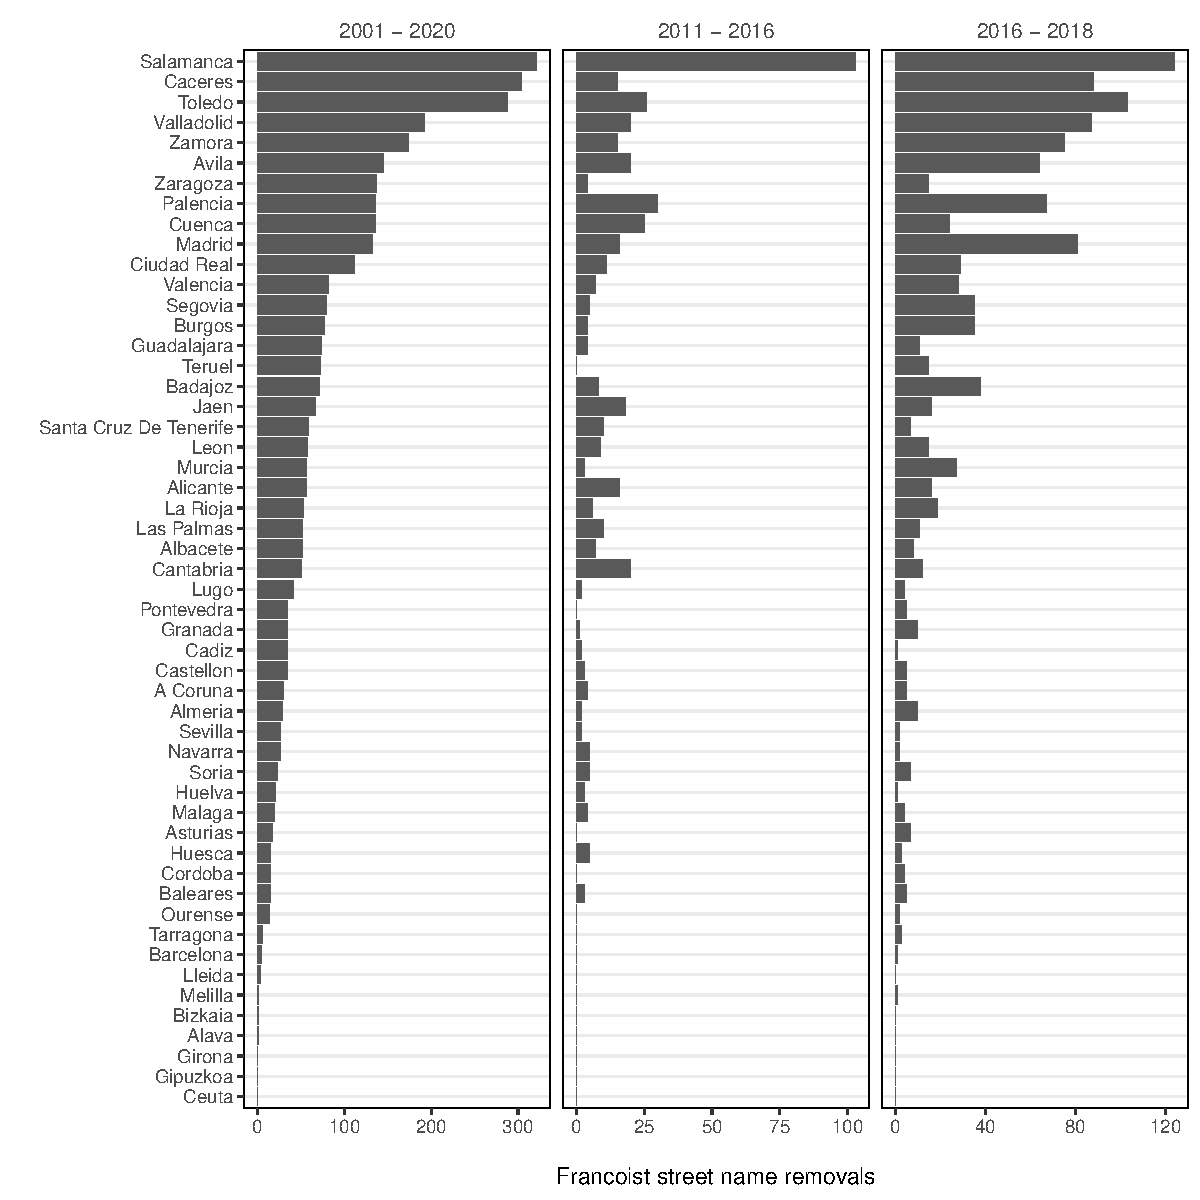
\includegraphics[width = \textwidth]{img/changes_by_prov}

  \caption{Number of Francoist street name removals over time}\label{fig:changes_by_prov}

\end{figure*}

\begin{figure*}[htb!]
\centering

  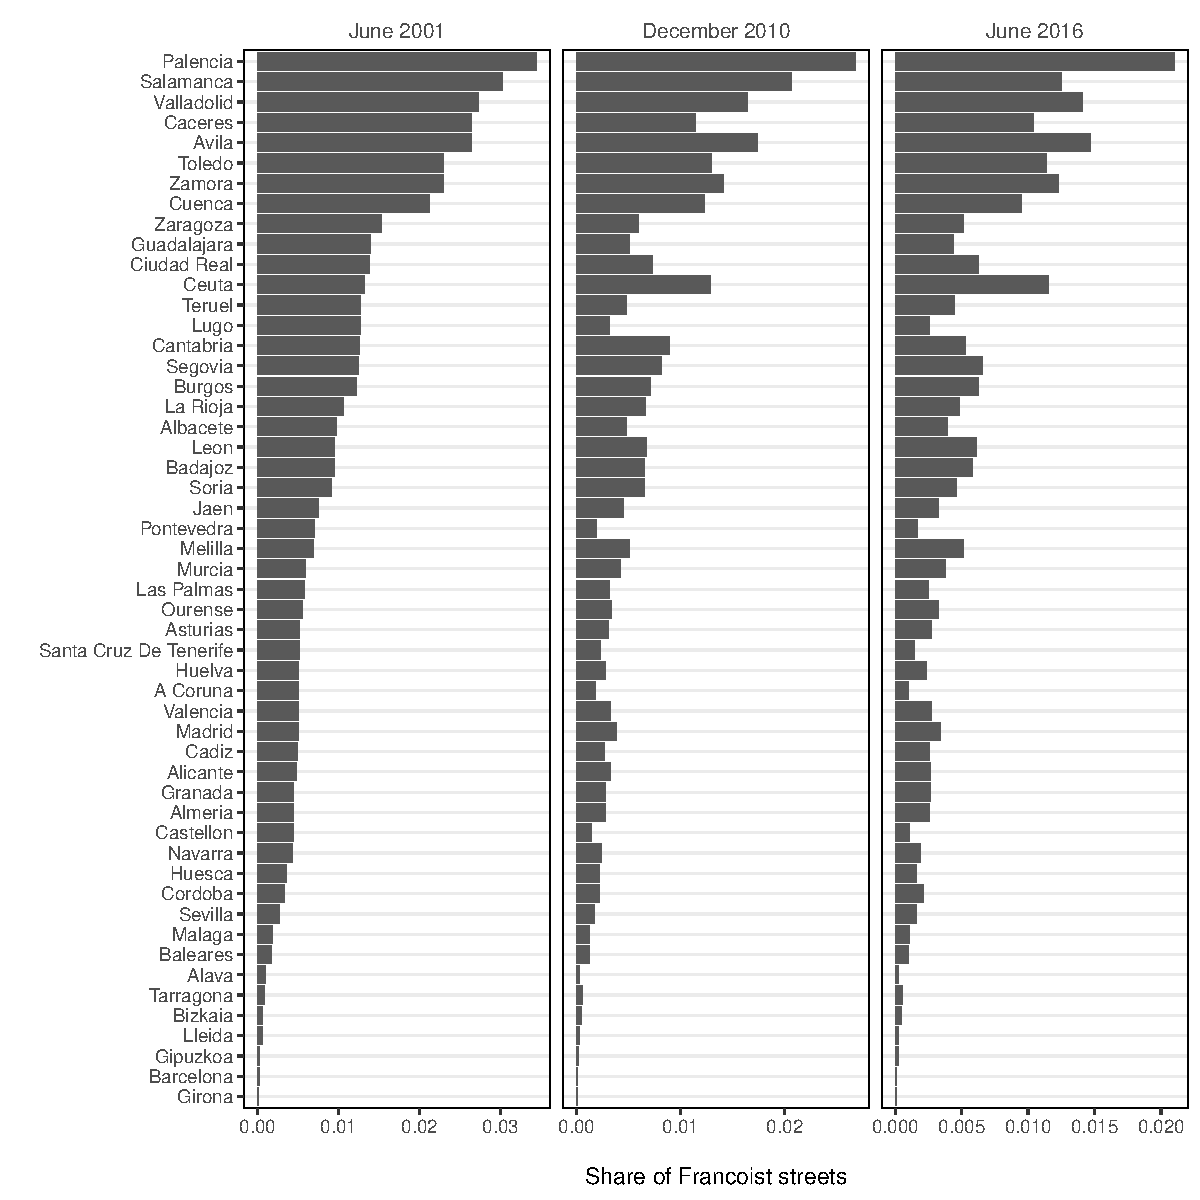
\includegraphics[width = \textwidth]{img/fs_by_prov}

  \caption{Share of Francoist streets in each province}\label{fig:fs_by_prov}

\end{figure*}

\clearpage
\section{Comparing treated vs control and sample vs out-of-sample}

One of the main concerns of the main analyses is that treated and control municipalities in the difference-in-differences analyses are not comparable.
To assess empirical evidence on this problem, table~\ref{tab:logit_fs_rm} shows the results of regressing a binary indicator of Francoist street name removal between 2016 and 2018 (the period covered in the DiD analyses in the main text) on a set of explanatory variable.
The sample only includes those municipalities that still had Francoist streets in June 2016.


% Table created by stargazer v.5.2.2 by Marek Hlavac, Harvard University. E-mail: hlavac at fas.harvard.edu
% Date and time: Tue, May 25, 2021 - 13:24:46
% Requires LaTeX packages: dcolumn 
\begin{table}[!htbp] \centering 
  \caption{Logit regression on Francoist street name removal (2016--2018)} 
  \label{tab:logit_fs_rm} 
\small 
\begin{tabular}{@{\extracolsep{-20pt}}lD{.}{.}{-3} D{.}{.}{-3} D{.}{.}{-3} } 
\\[-1.8ex]\hline 
\hline \\[-1.8ex] 
\\[-1.8ex] & \multicolumn{1}{c}{fs\_rm\_2016s2\_2018s2\_bin} & \multicolumn{1}{c}{fs\_rm\_2016s2\_2018s2\_bin} & \multicolumn{1}{c}{fs\_rm\_2016s2\_2018s2\_bin} \\ 
\\[-1.8ex] & \multicolumn{1}{c}{(1)} & \multicolumn{1}{c}{(2)} & \multicolumn{1}{c}{(3)}\\ 
\hline \\[-1.8ex] 
 (Intercept) & 0.326^{***} & 0.150^{*} & -0.289 \\ 
  & (0.044) & (0.062) & (0.206) \\ 
  Leftist mayor 2015 & -0.008 & 0.021 & 0.024 \\ 
  & (0.021) & (0.022) & (0.026) \\ 
  Log. Population 2011 & -0.051^{***} & -0.038^{***} & -0.030^{***} \\ 
  & (0.005) & (0.006) & (0.008) \\ 
  Log. No. Francoist streets June 2016 & 0.339^{***} & 0.328^{***} & 0.342^{***} \\ 
  & (0.023) & (0.024) & (0.027) \\ 
  PP support, June 2016 &  &  & 0.159 \\ 
  &  &  & (0.130) \\ 
  Vox support, June 2016 &  &  & -2.861 \\ 
  &  &  & (3.558) \\ 
  Turnout, June 2016 &  &  & 0.438^{+} \\ 
  &  &  & (0.229) \\ 
 \hline \\[-1.8ex] 
CCAA Fixed Effects & \multicolumn{1}{c}{No} & \multicolumn{1}{c}{Yes} & \multicolumn{1}{c}{Yes} \\ 
Observations & \multicolumn{1}{c}{1,636} & \multicolumn{1}{c}{1,636} & \multicolumn{1}{c}{1,167} \\ 
Log Likelihood & \multicolumn{1}{c}{-867.939} & \multicolumn{1}{c}{-841.697} & \multicolumn{1}{c}{-523.509} \\ 
Akaike Inf. Crit. & \multicolumn{1}{c}{1,743.879} & \multicolumn{1}{c}{1,727.394} & \multicolumn{1}{c}{1,091.019} \\ 
\hline 
\hline \\[-1.8ex] 
\multicolumn{4}{c}{\parbox[t]{0.75\textwidth}{\textit{Note:} + $p<0.1$; * $p<0.05$; ** $p<0.01$; *** $p<0.001$. Only including municipalities that had at least one street with Francoist names in June 2016.}} \\ 
\end{tabular} 
\end{table} 


The picture that emerges from these analyses is that it was mainly smaller municipalities with a high number of Francoist streets at the beginning of the period the ones that were more likely to remove Francoist street names.
Interestingly, neither the election of a leftist mayor in 2015 nor electoral support for Vox and PP in June 2016 elections show any significant relationship with being assigned into treatment.

Moreover, following figures~\ref{fig:changes_by_prov} and \ref{fig:fs_by_prov}, these municipalities were located mostly in the center of Spain.
These results are in line with the idea that municipalities that still had and changed street names during this period were probably the ones that had not done so because of political inaction and that, if anything, the selection bias goes against our main hypothesis.

The core idea of the selection bias is that the sample, because of still having Francoist street names as late as 2016, should be relatively more rightist that the overall sample of Spanish municipalities.
Table~\ref{tab:ttest_sample} shows the results of t-tests between municipalities in and out of the sample (i.e. having any Francoist street name in June 2016) on electoral share for PP, PSOE, and Vox in all elections between 2011 and 2019.
Interestingly, the data shows that although support for rightist parties was stronger among municipalities that still had Francoist street names in June 2016, support for the center-left PSOE was higher as well.
Probably, this is due to the fact that the sample is more likely to include municipalities in the central regions in Spain compared to peripheral regions, where the main two parties (PP and PSOE) have much less support (particularly in Catalonia and the Basque Country).

\begin{table}[!htbp] \centering
\caption{Mean comparison municipalities in/out of sample}
\label{tab:ttest_sample}
\small
\begin{tabular}{lcccc}
\\[-1.8ex]\hline
\hline \\[-1.8ex]
\\[-1.8ex]
Party & In sample & Out of sample & Diff In-Out (\%) & P-value \\
\hline \\[-1.8ex]
& \multicolumn{4}{c}{April 2019}\\
PP & 26.72\% & 23.95\% & 2.77 & 0.000*** \\
PSOE & 31.72\% & 28.04\% & 3.68 & 0.000*** \\
VOX & 12.31\% & 9.33\% & 2.97 & 0.000*** \\
\hline \\[-1.8ex]
& \multicolumn{4}{c}{June 2016}\\
PP & 44.42\% & 38.49\% & 5.94 & 0.000*** \\
PSOE & 27.21\% & 23.13\% & 4.08 & 0.000*** \\
VOX & 0.21\% & 0.2\% & 0.01 & 0.650 \\
\hline \\[-1.8ex]
& \multicolumn{4}{c}{December 2015}\\
PP & 40.34\% & 35.26\% & 5.08 & 0.000*** \\
PSOE & 27.86\% & 23.26\% & 4.6 & 0.000*** \\
VOX & 0.23\% & 0.22\% & 0 & 0.796 \\
\hline \\[-1.8ex]
& \multicolumn{4}{c}{November 2011}\\
PP & 54.87\% & 47.07\% & 7.8 & 0.000*** \\
PSOE & 31.23\% & 28.01\% & 3.23 & 0.000*** \\
\hline
\hline \\[-1.8ex]
\multicolumn{5}{c}{\parbox[t]{0.65\textwidth}{\textit{Note:} + $p<0.1$; * $p<0.05$; ** $p<0.01$; *** $p<0.001$.}}\\
\end{tabular}
\end{table}


In order to check this, table~\ref{tab:insample} shows results of logistic regression of electoral support for PP and PSOE on being in the sample (having Francoist street names in June 2016), including CCAA fixed effects and controlling for population.
In this case, the results are much more clear: municipalities in the sample show higher levels of electoral support for the right-wing PP.


% Table created by stargazer v.5.2.2 by Marek Hlavac, Harvard University. E-mail: hlavac at fas.harvard.edu
% Date and time: Thu, Jun 03, 2021 - 16:44:06
% Requires LaTeX packages: dcolumn 
\begin{table}[!htbp] \centering 
  \caption{Voting for PP/PSOE and being in the sample and having a Francoist street name in June 2016} 
  \label{tab:insample} 
\small 
\begin{tabular}{@{\extracolsep{-20pt}}lD{.}{.}{-3} D{.}{.}{-3} D{.}{.}{-3} D{.}{.}{-3} D{.}{.}{-3} D{.}{.}{-3} } 
\\[-1.8ex]\hline 
\hline \\[-1.8ex] 
\\[-1.8ex] & \multicolumn{1}{c}{(1)} & \multicolumn{1}{c}{(2)} & \multicolumn{1}{c}{(3)} & \multicolumn{1}{c}{(4)} & \multicolumn{1}{c}{(5)} & \multicolumn{1}{c}{(6)}\\ 
\hline \\[-1.8ex] 
 (Intercept) & -0.208^{***} & -0.183^{***} & -0.179^{***} & -0.246^{***} & -0.268^{***} & -0.248^{***} \\ 
  & (0.048) & (0.049) & (0.049) & (0.048) & (0.042) & (0.044) \\ 
  PP (2000/03) & 0.126^{*} &  &  &  &  &  \\ 
  & (0.052) &  &  &  &  &  \\ 
  PSOE (2000/03) & -0.149^{**} &  &  &  &  &  \\ 
  & (0.053) &  &  &  &  &  \\ 
  PP (2004/03) &  & 0.128^{*} &  &  &  &  \\ 
  &  & (0.054) &  &  &  &  \\ 
  PSOE (2004/03) &  & -0.200^{***} &  &  &  &  \\ 
  &  & (0.055) &  &  &  &  \\ 
  PP (2008/03) &  &  & 0.131^{*} &  &  &  \\ 
  &  &  & (0.056) &  &  &  \\ 
  PSOE (2008/03) &  &  & -0.197^{***} &  &  &  \\ 
  &  &  & (0.055) &  &  &  \\ 
  PP (2011/11) &  &  &  & 0.212^{***} &  &  \\ 
  &  &  &  & (0.051) &  &  \\ 
  PSOE (2011/11) &  &  &  & -0.157^{**} &  &  \\ 
  &  &  &  & (0.056) &  &  \\ 
  PP (2015/12) &  &  &  &  & 0.263^{***} &  \\ 
  &  &  &  &  & (0.045) &  \\ 
  PSOE (2015/12) &  &  &  &  & -0.138^{**} &  \\ 
  &  &  &  &  & (0.054) &  \\ 
  PP (2016/06) &  &  &  &  &  & 0.237^{***} \\ 
  &  &  &  &  &  & (0.046) \\ 
  PSOE (2016/06) &  &  &  &  &  & -0.175^{**} \\ 
  &  &  &  &  &  & (0.057) \\ 
  Log. Pop 2011 & 0.073^{***} & 0.076^{***} & 0.074^{***} & 0.072^{***} & 0.075^{***} & 0.074^{***} \\ 
  & (0.003) & (0.003) & (0.003) & (0.003) & (0.003) & (0.003) \\ 
 \hline \\[-1.8ex] 
CCAA Fixed Effects & \multicolumn{1}{c}{Yes} & \multicolumn{1}{c}{Yes} & \multicolumn{1}{c}{Yes} & \multicolumn{1}{c}{Yes} & \multicolumn{1}{c}{Yes} & \multicolumn{1}{c}{Yes} \\ 
Observations & \multicolumn{1}{c}{7,593} & \multicolumn{1}{c}{7,890} & \multicolumn{1}{c}{7,893} & \multicolumn{1}{c}{7,897} & \multicolumn{1}{c}{7,897} & \multicolumn{1}{c}{7,897} \\ 
Akaike Inf. Crit. & \multicolumn{1}{c}{6,625.822} & \multicolumn{1}{c}{6,839.057} & \multicolumn{1}{c}{6,837.529} & \multicolumn{1}{c}{6,829.387} & \multicolumn{1}{c}{6,830.442} & \multicolumn{1}{c}{6,827.124} \\ 
\hline 
\hline \\[-1.8ex] 
\multicolumn{7}{c}{\parbox[t]{0.6\textwidth}{\textit{Note:} $+ p<0.1; * p<0.05; ** p<0.01; *** p<0.001$.}} \\ 
\end{tabular} 
\end{table} 


Going further back in time, table~\ref{tab:ttest_sample2001} and table~\ref{tab:insample2001} repeat these analyses but distinguishing between municipalities that had ir did not have Francoist street names in June 2001, the earliest point in time for which we have available data.
Moreover, we use data on all elections since 2000.
Again, the same patterns emerge.
Municipalities that had Francoist street names in later periods were more, on average, more rightist, or at least supported PP stronger.

\begin{table}[!htbp] \centering
\caption{Mean comparison municipalities with/without Francoist street names in June 2001}
\label{tab:ttest_sample2001}
\small
\begin{tabular}{lcccc}
\\[-1.8ex]\hline
\hline \\[-1.8ex]
\\[-1.8ex]
Party & In sample & Out of sample & Diff In-Out (\%) & P-value \\
\hline \\[-1.8ex]
& \multicolumn{4}{c}{April 2019}\\
PP & 27.23\% & 23.47\% & 3.75 & 0.000*** \\
PSOE & 31.53\% & 27.75\% & 3.77 & 0.000*** \\
VOX & 12.22\% & 9.08\% & 3.15 & 0.000*** \\
\hline \\[-1.8ex]
& \multicolumn{4}{c}{June 2016}\\
PP & 44.85\% & 37.74\% & 7.11 & 0.000*** \\
PSOE & 26.9\% & 22.86\% & 4.04 & 0.000*** \\
VOX & 0.21\% & 0.2\% & 0.02 & 0.278 \\
\hline \\[-1.8ex]
& \multicolumn{4}{c}{December 2015}\\
PP & 40.85\% & 34.57\% & 6.28 & 0.000*** \\
PSOE & 27.5\% & 22.95\% & 4.55 & 0.000*** \\
VOX & 0.24\% & 0.22\% & 0.02 & 0.260 \\
\hline \\[-1.8ex]
& \multicolumn{4}{c}{November 2011}\\
PP & 55.17\% & 46.2\% & 8.96 & 0.000*** \\
PSOE & 31\% & 27.78\% & 3.21 & 0.000*** \\
\hline \\[-1.8ex]
& \multicolumn{4}{c}{March 2008}\\
PP & 48.65\% & 41.07\% & 7.58 & 0.000*** \\
PSOE & 42.99\% & 39.63\% & 3.37 & 0.000*** \\
\hline \\[-1.8ex]
& \multicolumn{4}{c}{March 2004}\\
PP & 48.49\% & 41.57\% & 6.92 & 0.000*** \\
PSOE & 42.09\% & 36.68\% & 5.41 & 0.000*** \\
\hline \\[-1.8ex]
& \multicolumn{4}{c}{March 2000}\\
PP & 53.18\% & 46.81\% & 6.37 & 0.000*** \\
PSOE & 36.21\% & 31.46\% & 4.74 & 0.000*** \\
\hline
\hline \\[-1.8ex]
\multicolumn{5}{c}{\parbox[t]{0.65\textwidth}{\textit{Note:} * $p<0.05$; ** $p<0.01$; *** $p<0.001$.}}\\
\end{tabular}
\end{table}


% Table created by stargazer v.5.2.2 by Marek Hlavac, Harvard University. E-mail: hlavac at fas.harvard.edu
% Date and time: Fri, May 28, 2021 - 12:24:32
% Requires LaTeX packages: dcolumn 
\begin{table}[!htbp] \centering 
  \caption{Voting for PP/PSOE and being in the sample and having a Francoist street name in June 2001} 
  \label{tab:insample2001} 
\small 
\begin{tabular}{@{\extracolsep{-20pt}}lD{.}{.}{-3} D{.}{.}{-3} D{.}{.}{-3} D{.}{.}{-3} D{.}{.}{-3} D{.}{.}{-3} } 
\\[-1.8ex]\hline 
\hline \\[-1.8ex] 
\\[-1.8ex] & \multicolumn{1}{c}{(1)} & \multicolumn{1}{c}{(2)} & \multicolumn{1}{c}{(3)} & \multicolumn{1}{c}{(4)} & \multicolumn{1}{c}{(5)} & \multicolumn{1}{c}{(6)}\\ 
\hline \\[-1.8ex] 
 (Intercept) & -0.269^{***} & -0.252^{***} & -0.231^{***} & -0.338^{***} & -0.328^{***} & -0.305^{***} \\ 
  & (0.052) & (0.053) & (0.054) & (0.053) & (0.047) & (0.048) \\ 
  PP (2000/03) & 0.234^{***} &  &  &  &  &  \\ 
  & (0.056) &  &  &  &  &  \\ 
  PSOE (2000/03) & -0.083 &  &  &  &  &  \\ 
  & (0.058) &  &  &  &  &  \\ 
  PP (2004/03) &  & 0.239^{***} &  &  &  &  \\ 
  &  & (0.059) &  &  &  &  \\ 
  PSOE (2004/03) &  & -0.125^{*} &  &  &  &  \\ 
  &  & (0.061) &  &  &  &  \\ 
  PP (2008/03) &  &  & 0.205^{***} &  &  &  \\ 
  &  &  & (0.061) &  &  &  \\ 
  PSOE (2008/03) &  &  & -0.126^{*} &  &  &  \\ 
  &  &  & (0.061) &  &  &  \\ 
  PP (2011/11) &  &  &  & 0.340^{***} &  &  \\ 
  &  &  &  & (0.056) &  &  \\ 
  PSOE (2011/11) &  &  &  & -0.047 &  &  \\ 
  &  &  &  & (0.062) &  &  \\ 
  PP (2015/12) &  &  &  &  & 0.358^{***} &  \\ 
  &  &  &  &  & (0.050) &  \\ 
  PSOE (2015/12) &  &  &  &  & -0.066 &  \\ 
  &  &  &  &  & (0.059) &  \\ 
  PP (2016/06) &  &  &  &  &  & 0.327^{***} \\ 
  &  &  &  &  &  & (0.051) \\ 
  PSOE (2016/06) &  &  &  &  &  & -0.105^{+} \\ 
  &  &  &  &  &  & (0.063) \\ 
  Log. Pop 2011 & 0.078^{***} & 0.081^{***} & 0.079^{***} & 0.077^{***} & 0.082^{***} & 0.080^{***} \\ 
  & (0.003) & (0.003) & (0.003) & (0.003) & (0.003) & (0.003) \\ 
 \hline \\[-1.8ex] 
CCAA Fixed Effects & \multicolumn{1}{c}{Yes} & \multicolumn{1}{c}{Yes} & \multicolumn{1}{c}{Yes} & \multicolumn{1}{c}{Yes} & \multicolumn{1}{c}{Yes} & \multicolumn{1}{c}{Yes} \\ 
Observations & \multicolumn{1}{c}{7,593} & \multicolumn{1}{c}{7,890} & \multicolumn{1}{c}{7,893} & \multicolumn{1}{c}{7,897} & \multicolumn{1}{c}{7,897} & \multicolumn{1}{c}{7,897} \\ 
Akaike Inf. Crit. & \multicolumn{1}{c}{8,001.884} & \multicolumn{1}{c}{8,353.067} & \multicolumn{1}{c}{8,365.240} & \multicolumn{1}{c}{8,343.314} & \multicolumn{1}{c}{8,342.123} & \multicolumn{1}{c}{8,342.252} \\ 
\hline 
\hline \\[-1.8ex] 
\multicolumn{7}{c}{\parbox[t]{0.6\textwidth}{\textit{Note:} $+ p<0.1; * p<0.05; ** p<0.01; *** p<0.001$.}} \\ 
\end{tabular} 
\end{table} 


\clearpage
\section{Additional cross-sectional analysis}

Table~\ref{tab:cs_change} shows the results of cross-sectional analyses similar to the ones shown in the main text but using the change in support for Vox between April and November 2019 as the dependent variable.
As discussed in the main text, these results that any effect of the removal of Francoist streets took place between the April 2019 elections.


% Table created by stargazer v.5.2.2 by Marek Hlavac, Harvard University. E-mail: hlavac at fas.harvard.edu
% Date and time: Wed, Oct 06, 2021 - 13:08:27
% Requires LaTeX packages: dcolumn 
\begin{table}[!htbp] \centering 
  \caption{Francoist street name removal and change in electoral support for Vox during 2019} 
  \label{tab:cs_change} 
\small 
\begin{tabular}{@{\extracolsep{-20pt}}lD{.}{.}{-3} D{.}{.}{-3} } 
\\[-1.8ex]\hline 
\hline \\[-1.8ex] 
\\[-1.8ex] & \multicolumn{1}{c}{\footnotesize Full sample} & \multicolumn{1}{c}{\footnotesize Limited sample} \\ 
\\[-1.8ex] & \multicolumn{1}{c}{(1)} & \multicolumn{1}{c}{(2)}\\ 
\hline \\[-1.8ex] 
 (Intercept) & 2.195^{***} & 2.362^{***} \\ 
  & (0.119) & (0.156) \\ 
  Francoist street name removal & -0.015 & 0.003 \\ 
  & (0.020) & (0.019) \\ 
  Unemployment 2019 & 0.518 & 0.450 \\ 
  & (0.337) & (0.404) \\ 
  Turnout April 2019 & -0.623^{***} & -0.799^{***} \\ 
  & (0.133) & (0.178) \\ 
  Turnout Nov 2019 & -0.009^{+} & -0.018^{**} \\ 
  & (0.005) & (0.006) \\ 
 \hline \\[-1.8ex] 
CCAA Fixed Effects & \multicolumn{1}{c}{Yes} & \multicolumn{1}{c}{Yes} \\ 
Observations & \multicolumn{1}{c}{7,552} & \multicolumn{1}{c}{2,153} \\ 
R$^{2}$ & \multicolumn{1}{c}{0.078} & \multicolumn{1}{c}{0.134} \\ 
Adjusted R$^{2}$ & \multicolumn{1}{c}{0.075} & \multicolumn{1}{c}{0.125} \\ 
\hline 
\hline \\[-1.8ex] 
\multicolumn{3}{c}{\parbox[t]{0.6\textwidth}{\textit{Note:} $+ p<0.1; * p<0.05; ** p<0.01; *** p<0.001$. The main independent variable refers to the removal of Francoist street names between June 2001 and December 2018. The limited sample corresponds to municipalities that had Francoist street names in June 2001.}} \\ 
\end{tabular} 
\end{table} 


Tables~\ref{tab:cs_all_2011} and \ref{tab:cs_limited_2011} replicate the analyses in the main text---plus the model using the change between April and November as dependent variable---using as independent variable the removal of Francoist streets between 2011 and 2018, using the full and limited samples, respectively.
Results point in the same direction as the cross-sectional models in the main text, that is, the removal of Francoist street names is correlated with the increase in support for Vox between 2016 and 2019.


% Table created by stargazer v.5.2.2 by Marek Hlavac, Harvard University. E-mail: hlavac at fas.harvard.edu
% Date and time: Fri, Jun 11, 2021 - 14:03:35
% Requires LaTeX packages: dcolumn 
\begin{table}[!htbp] \centering 
  \caption{Electoral support for Vox and Francoist street name removal (2011--2018)} 
  \label{tab:cs_all_2011} 
\small 
\begin{tabular}{@{\extracolsep{-20pt}}lD{.}{.}{-3} D{.}{.}{-3} D{.}{.}{-3} } 
\\[-1.8ex]\hline 
\hline \\[-1.8ex] 
\\[-1.8ex] & \multicolumn{1}{c}{\footnotesize Apr 2019} & \multicolumn{1}{c}{\footnotesize Nov 2019} & \multicolumn{1}{c}{\footnotesize Change} \\ 
\\[-1.8ex] & \multicolumn{1}{c}{(1)} & \multicolumn{1}{c}{(2)} & \multicolumn{1}{c}{(3)}\\ 
\hline \\[-1.8ex] 
 (Intercept) & 0.078^{***} & 0.145^{***} & 2.197^{***} \\ 
  & (0.009) & (0.010) & (0.119) \\ 
  Francoist street name removal & 0.010^{***} & 0.013^{***} & -0.011 \\ 
  & (0.002) & (0.002) & (0.026) \\ 
  Unemployment 2019 & 0.083^{***} & 0.195^{***} & 0.517 \\ 
  & (0.025) & (0.031) & (0.337) \\ 
  Turnout April 2019 & 0.005 &  & -0.623^{***} \\ 
  & (0.010) &  & (0.133) \\ 
  Turnout Nov 2019 &  & -0.037^{***} &  \\ 
  &  & (0.011) &  \\ 
  Log. Population & 0.003^{***} & 0.006^{***} & -0.009^{+} \\ 
  & (0.000) & (0.000) & (0.005) \\ 
 \hline \\[-1.8ex] 
CCAA Fixed Effects & \multicolumn{1}{c}{Yes} & \multicolumn{1}{c}{Yes} & \multicolumn{1}{c}{Yes} \\ 
Observations & \multicolumn{1}{c}{7,819} & \multicolumn{1}{c}{7,820} & \multicolumn{1}{c}{7,552} \\ 
R$^{2}$ & \multicolumn{1}{c}{0.441} & \multicolumn{1}{c}{0.499} & \multicolumn{1}{c}{0.078} \\ 
Adjusted R$^{2}$ & \multicolumn{1}{c}{0.440} & \multicolumn{1}{c}{0.497} & \multicolumn{1}{c}{0.075} \\ 
\hline 
\hline \\[-1.8ex] 
\multicolumn{4}{c}{\parbox[t]{0.7\textwidth}{\textit{Note:} $+ p<0.1; * p<0.05; ** p<0.01; *** p<0.001$. The main independent variable refers to the removal of Francoist street names between December 2010 and December 2018.}} \\ 
\end{tabular} 
\end{table} 


% Table created by stargazer v.5.2.2 by Marek Hlavac, Harvard University. E-mail: hlavac at fas.harvard.edu
% Date and time: Tue, May 25, 2021 - 14:21:10
% Requires LaTeX packages: dcolumn 
\begin{table}[!htbp] \centering 
  \caption{Electoral support for Vox and Francoist street name removal} 
  \label{tab:cs_limited_2011} 
\small 
\begin{tabular}{@{\extracolsep{-20pt}}lD{.}{.}{-3} D{.}{.}{-3} D{.}{.}{-3} } 
\\[-1.8ex]\hline 
\hline \\[-1.8ex] 
\\[-1.8ex] & \multicolumn{1}{c}{\footnotesize Apr 2019} & \multicolumn{1}{c}{\footnotesize Nov 2019} & \multicolumn{1}{c}{\footnotesize Change} \\ 
\\[-1.8ex] & \multicolumn{1}{c}{(1)} & \multicolumn{1}{c}{(2)} & \multicolumn{1}{c}{(3)}\\ 
\hline \\[-1.8ex] 
 (Intercept) & 0.115^{***} & 0.218^{***} & 2.476^{***} \\ 
  & (0.020) & (0.022) & (0.174) \\ 
  Francoist street name removal & 0.006^{*} & 0.007^{*} & -0.012 \\ 
  & (0.002) & (0.003) & (0.022) \\ 
  Unemployment 2019 & 0.002 & 0.097 & 0.381 \\ 
  & (0.051) & (0.062) & (0.443) \\ 
  Turnout April 2019 & -0.012 &  & -0.901^{***} \\ 
  & (0.023) &  & (0.200) \\ 
  Turnout Nov 2019 &  & -0.088^{***} &  \\ 
  &  & (0.025) &  \\ 
  Log. Population & 0.002^{*} & 0.003^{***} & -0.023^{**} \\ 
  & (0.001) & (0.001) & (0.007) \\ 
 \hline \\[-1.8ex] 
CCAA Fixed Effects & \multicolumn{1}{c}{Yes} & \multicolumn{1}{c}{Yes} & \multicolumn{1}{c}{Yes} \\ 
Observations & \multicolumn{1}{c}{1,791} & \multicolumn{1}{c}{1,792} & \multicolumn{1}{c}{1,782} \\ 
R$^{2}$ & \multicolumn{1}{c}{0.269} & \multicolumn{1}{c}{0.296} & \multicolumn{1}{c}{0.129} \\ 
Adjusted R$^{2}$ & \multicolumn{1}{c}{0.260} & \multicolumn{1}{c}{0.287} & \multicolumn{1}{c}{0.118} \\ 
\hline 
\hline \\[-1.8ex] 
\multicolumn{4}{c}{\parbox[t]{0.7\textwidth}{\textit{Note:} $+ p<0.1; * p<0.05; ** p<0.01; *** p<0.001$. The main independent variable refers to the removal of Francoist street names between December 2010 and December 2018. Only municipalities that had Francoist street names in June 2011 were included.}} \\ 
\end{tabular} 
\end{table} 


Finally, for comparison, table~\ref{tab:cs_periods} repeats the cross-sectional analyses but including the main independent variable (the removal of Francoist street names) for different periods, using support for Vox as our dependent variable.
In particular, we include street name removals between 2001 and 2015 (\textit{before} our study period), 2001 and 2018 (full period), 2011 and 2018, and 2016 and 2018 (same period as in the main analyses).
We only include municipalities that had Francoist street names at the beginning of each period.
The results show that the removal of Francoist street names only has a significant correlation with support for Vox when recent name removals are included, i.e., when the independent variable includes removals in 2016 and after.


% Table created by stargazer v.5.2.2 by Marek Hlavac, Harvard University. E-mail: hlavac at fas.harvard.edu
% Date and time: Wed, Oct 06, 2021 - 13:08:27
% Requires LaTeX packages: dcolumn 
\begin{table}[!htbp] \centering 
  \caption{Electoral support for Vox in 2019 and Francoist street name removal across different periods} 
  \label{tab:cs_periods} 
\small 
\begin{tabular}{@{\extracolsep{-20pt}}lD{.}{.}{-3} D{.}{.}{-3} D{.}{.}{-3} D{.}{.}{-3} } 
\\[-1.8ex]\hline 
\hline \\[-1.8ex] 
\\[-1.8ex] & \multicolumn{1}{c}{2001-2015} & \multicolumn{1}{c}{2001-2018} & \multicolumn{1}{c}{2011-2018} & \multicolumn{1}{c}{2016-2018} \\ 
\\[-1.8ex] & \multicolumn{1}{c}{(1)} & \multicolumn{1}{c}{(2)} & \multicolumn{1}{c}{(3)} & \multicolumn{1}{c}{(4)}\\ 
\hline \\[-1.8ex] 
 (Intercept) & 0.120^{***} & 0.119^{***} & 0.115^{***} & 0.118^{***} \\ 
  & (0.018) & (0.018) & (0.020) & (0.021) \\ 
  Francoist street name removal & 0.003 & 0.005^{*} & 0.006^{*} & 0.007^{*} \\ 
  & (0.002) & (0.002) & (0.002) & (0.003) \\ 
  Unemployment 2019 & 0.045 & 0.043 & 0.002 & -0.031 \\ 
  & (0.047) & (0.047) & (0.051) & (0.053) \\ 
  Turnout April 2019 & -0.020 & -0.020 & -0.012 & -0.020 \\ 
  & (0.021) & (0.020) & (0.023) & (0.024) \\ 
  Log. Population & 0.001^{+} & 0.002^{*} & 0.002^{*} & 0.003^{**} \\ 
  & (0.001) & (0.001) & (0.001) & (0.001) \\ 
 \hline \\[-1.8ex] 
CCAA Fixed Effects & \multicolumn{1}{c}{Yes} & \multicolumn{1}{c}{Yes} & \multicolumn{1}{c}{Yes} & \multicolumn{1}{c}{Yes} \\ 
Observations & \multicolumn{1}{c}{2,164} & \multicolumn{1}{c}{2,164} & \multicolumn{1}{c}{1,791} & \multicolumn{1}{c}{1,611} \\ 
R$^{2}$ & \multicolumn{1}{c}{0.290} & \multicolumn{1}{c}{0.292} & \multicolumn{1}{c}{0.269} & \multicolumn{1}{c}{0.264} \\ 
Adjusted R$^{2}$ & \multicolumn{1}{c}{0.283} & \multicolumn{1}{c}{0.284} & \multicolumn{1}{c}{0.260} & \multicolumn{1}{c}{0.254} \\ 
\hline 
\hline \\[-1.8ex] 
\multicolumn{5}{c}{\parbox[t]{0.7\textwidth}{\textit{Note:} $+ p<0.1; * p<0.05; ** p<0.01; *** p<0.001$. The main independent variable refers to the removal of Francoist street names in different periods: 1) June 2001 - December 2015, 2) June 2001 - December 2018, 3) December 2010 - December 2018, and 4) June 2016 - December 2018. Only municipalities that had Francoist street names at the beginning of each period were included.}} \\ 
\end{tabular} 
\end{table} 


\clearpage
\section{Robustness tests (difference-in-differences)}

Table~\ref{tab:vox_robustness} shows the robustness tests for the DiD analyses using electoral support for Vox as the dependent variable, while tables~\ref{tab:pp_robustness} and \ref{tab:psoe_robustness} do the same but using PP and PSOE share, respectively, as the dependent variable.
All models in these tables include elections before June 2016: December 2015 in the case of Vox, and all elections since March 2000 for PP and PSOE.
Model 2 extends the dependent variable to the first half of 2019, accounting for potential delays in the registration of name changes that could have affected electoral support in April 2019.
Model 3 uses the independent variable in continuous form, namely, the logged number of street name removals.
Model 4 restricts the sample to municipalities where Vox got more than 0 votes in 2016 elections, to account for potential estimation issues.

The two main takeaways from these results is that the main result does not change across the different specifications and that the parallel trend assumption holds.
In the case of Vox, the pre-treatment DiD estimate (December 2015) does not show any statistical significance, while in the case of PP none of the DiD estimates between March 2000 and December 2015 in any of the models is significant either.
In the PSOE models, it seems that municipalities that later removed Francoist names showed more support for the PSOE in earlier elections (November 2011 and December 2015), but this result is not robust across all specifications.

Finally, table~\ref{tab:models_se} repeats the main analyses for PP and Vox using normal standard errors, heteroskedasticity-consistent standard errors, and standard errors clustered at the level of municipalities.
Although levels of significance go down in the case of Vox, it still retain statistical significance and, in the case of PP, significance increases.


% Table created by stargazer v.5.2.2 by Marek Hlavac, Harvard University. E-mail: hlavac at fas.harvard.edu
% Date and time: Thu, May 27, 2021 - 19:57:41
% Requires LaTeX packages: dcolumn 
\begin{table}[!htbp] \centering 
  \caption{Francoist street name removal and increase in electoral support for Vox} 
  \label{tab:vox_robustness} 
\small 
\begin{tabular}{@{\extracolsep{-20pt}}lD{.}{.}{-3} D{.}{.}{-3} D{.}{.}{-3} D{.}{.}{-3} } 
\\[-1.8ex]\hline 
\hline \\[-1.8ex] 
\\[-1.8ex] & \multicolumn{1}{c}{(1)} & \multicolumn{1}{c}{(2)} & \multicolumn{1}{c}{(3)} & \multicolumn{1}{c}{(4)}\\ 
\hline \\[-1.8ex] 
 (Intercept) & -0.968^{**} & -0.969^{**} & -0.929^{**} & 0.127 \\ 
  & (0.326) & (0.326) & (0.324) & (0.399) \\ 
  Francoist street name removal & -0.078 & -0.066 & -0.163 & -0.231 \\ 
  & (0.220) & (0.215) & (0.188) & (0.253) \\ 
  Election December 2015 & -0.101 & -0.102 & -0.109 & -0.119 \\ 
  & (0.148) & (0.149) & (0.144) & (0.159) \\ 
  Election April 2019 & 12.319^{***} & 12.305^{***} & 12.300^{***} & 12.898^{***} \\ 
  & (0.142) & (0.144) & (0.139) & (0.153) \\ 
  Francoist removal $\times$ Dec 2015 & -0.019 & -0.011 & 0.021 & -0.048 \\ 
  & (0.314) & (0.306) & (0.253) & (0.362) \\ 
  Francoist removal $\times$ April 2019 & 0.724^{*} & 0.735^{*} & 0.746^{**} & 0.789^{*} \\ 
  & (0.299) & (0.293) & (0.244) & (0.347) \\ 
 \hline \\[-1.8ex] 
Controls & \multicolumn{1}{c}{Yes} & \multicolumn{1}{c}{Yes} & \multicolumn{1}{c}{Yes} & \multicolumn{1}{c}{Yes} \\ 
CCAA Fixed Effects & \multicolumn{1}{c}{Yes} & \multicolumn{1}{c}{Yes} & \multicolumn{1}{c}{Yes} & \multicolumn{1}{c}{Yes} \\ 
Observations & \multicolumn{1}{c}{3,303} & \multicolumn{1}{c}{3,303} & \multicolumn{1}{c}{3,303} & \multicolumn{1}{c}{2,259} \\ 
R$^{2}$ & \multicolumn{1}{c}{0.802} & \multicolumn{1}{c}{0.802} & \multicolumn{1}{c}{0.802} & \multicolumn{1}{c}{0.844} \\ 
Adjusted R$^{2}$ & \multicolumn{1}{c}{0.801} & \multicolumn{1}{c}{0.801} & \multicolumn{1}{c}{0.801} & \multicolumn{1}{c}{0.843} \\ 
\hline 
\hline \\[-1.8ex] 
\multicolumn{5}{c}{\parbox[t]{0.85\textwidth}{\textit{Note:} + $p<0.1$; * $p<0.05$; ** $p<0.01$; *** $p<0.001$. All models also include elections before June 2016 (December 2015). Model 2 extends the DV (name removal) to the first half of 2019. Model 3 uses the IV in continuous form (logged number of changes). Model 4 restricts the sample to municipalities where Vox got more than 0 votes. Controls include a dummy for a leftist major elected in 2015 local elections, logged population in 2011, logged number of Francoist streets in $t_{0}$, and the unemployment rate in January 2016. Only municipalities that had at least one street with a Francoist name in $t_{0}$ (June 2016) were included in the sample.}} \\ 
\end{tabular} 
\end{table} 


% Table created by stargazer v.5.2.2 by Marek Hlavac, Harvard University. E-mail: hlavac at fas.harvard.edu
% Date and time: Tue, Jun 15, 2021 - 19:16:26
% Requires LaTeX packages: dcolumn 
\begin{table}[!htbp] \centering 
  \caption{Francoist street name removal and change in electoral support for PP} 
  \label{tab:pp_robustness} 
\small 
\begin{tabular}{@{\extracolsep{-20pt}}lD{.}{.}{-3} D{.}{.}{-3} D{.}{.}{-3} D{.}{.}{-3} } 
\\[-1.8ex]\hline 
\hline \\[-1.8ex] 
\\[-1.8ex] & \multicolumn{1}{c}{(1)} & \multicolumn{1}{c}{(2)} & \multicolumn{1}{c}{(3)} & \multicolumn{1}{c}{(4)}\\ 
\hline \\[-1.8ex] 
 (Intercept) & 49.323^{***} & 49.312^{***} & 49.484^{***} & 43.384^{***} \\ 
  & (0.593) & (0.594) & (0.589) & (0.751) \\ 
  Francoist street name removal & 1.009^{*} & 0.974^{+} & 0.841^{+} & 0.634 \\ 
  & (0.511) & (0.502) & (0.436) & (0.695) \\ 
  Election March 2000 & 8.091^{***} & 8.015^{***} & 8.132^{***} & 8.539^{***} \\ 
  & (0.374) & (0.379) & (0.363) & (0.428) \\ 
  Election March 2004 & 3.291^{***} & 3.273^{***} & 3.310^{***} & 3.614^{***} \\ 
  & (0.374) & (0.379) & (0.363) & (0.428) \\ 
  Election March 2008 & 4.267^{***} & 4.264^{***} & 4.218^{***} & 6.074^{***} \\ 
  & (0.374) & (0.379) & (0.363) & (0.428) \\ 
  Election November 2011 & 10.569^{***} & 10.561^{***} & 10.538^{***} & 12.127^{***} \\ 
  & (0.374) & (0.379) & (0.363) & (0.428) \\ 
  Election December 2015 & -4.075^{***} & -4.063^{***} & -4.039^{***} & -4.218^{***} \\ 
  & (0.374) & (0.379) & (0.363) & (0.428) \\ 
  Election April 2019 & -17.382^{***} & -17.343^{***} & -17.379^{***} & -17.657^{***} \\ 
  & (0.376) & (0.381) & (0.364) & (0.428) \\ 
  Francoist removal $\times$ March 2000 & -0.106 & 0.161 & -0.241 & 0.132 \\ 
  & (0.711) & (0.698) & (0.594) & (0.970) \\ 
  Francoist removal $\times$ March 2004 & 0.741 & 0.754 & 0.634 & 0.674 \\ 
  & (0.711) & (0.697) & (0.594) & (0.970) \\ 
  Francoist removal $\times$ March 2008 & -0.631 & -0.581 & -0.430 & -0.087 \\ 
  & (0.711) & (0.697) & (0.594) & (0.970) \\ 
  Francoist removal $\times$ Nov 2011 & -0.425 & -0.369 & -0.295 & 0.040 \\ 
  & (0.711) & (0.697) & (0.594) & (0.970) \\ 
  Francoist removal $\times$ Dec 2015 & -0.007 & -0.049 & -0.132 & -0.158 \\ 
  & (0.711) & (0.697) & (0.594) & (0.970) \\ 
  Francoist removal $\times$ April 2019 & -1.422^{*} & -1.466^{*} & -1.352^{*} & -1.781^{+} \\ 
  & (0.712) & (0.699) & (0.594) & (0.970) \\ 
 \hline \\[-1.8ex] 
Controls & \multicolumn{1}{c}{Yes} & \multicolumn{1}{c}{Yes} & \multicolumn{1}{c}{Yes} & \multicolumn{1}{c}{Yes} \\ 
CCAA Fixed Effects & \multicolumn{1}{c}{Yes} & \multicolumn{1}{c}{Yes} & \multicolumn{1}{c}{Yes} & \multicolumn{1}{c}{Yes} \\ 
Observations & \multicolumn{1}{c}{11,325} & \multicolumn{1}{c}{11,325} & \multicolumn{1}{c}{11,325} & \multicolumn{1}{c}{5,502} \\ 
R$^{2}$ & \multicolumn{1}{c}{0.683} & \multicolumn{1}{c}{0.683} & \multicolumn{1}{c}{0.683} & \multicolumn{1}{c}{0.718} \\ 
Adjusted R$^{2}$ & \multicolumn{1}{c}{0.682} & \multicolumn{1}{c}{0.682} & \multicolumn{1}{c}{0.682} & \multicolumn{1}{c}{0.717} \\ 
\hline 
\hline \\[-1.8ex] 
\multicolumn{5}{c}{\parbox[t]{0.85\textwidth}{\textit{Note:} + $p<0.1$; * $p<0.05$; ** $p<0.01$; *** $p<0.001$. All models also include elections before June 2016 (2000--2015). Model 2 extends the DV (name removal) to the first half of 2019. Model 3 uses the IV in continuous form (logged number of changes). Model 4 restricts the sample to municipalities where Vox got more than 0 votes. Controls include a dummy for a leftist major elected in 2015 local elections, logged population in 2011, logged number of Francoist streets in $t_{0}$, and the unemployment rate in January 2016. Only municipalities that had at least one street with a Francoist name in $t_{0}$ (June 2016) were included in the sample.}} \\ 
\end{tabular} 
\end{table} 


% Table created by stargazer v.5.2.2 by Marek Hlavac, Harvard University. E-mail: hlavac at fas.harvard.edu
% Date and time: Thu, May 27, 2021 - 19:57:42
% Requires LaTeX packages: dcolumn 
\begin{table}[!htbp] \centering 
  \caption{Francoist street name removal and increase in electoral support for PSOE} 
  \label{tab:PSOE_robustness} 
\small 
\begin{tabular}{@{\extracolsep{-20pt}}lD{.}{.}{-3} D{.}{.}{-3} D{.}{.}{-3} D{.}{.}{-3} } 
\\[-1.8ex]\hline 
\hline \\[-1.8ex] 
\\[-1.8ex] & \multicolumn{1}{c}{(1)} & \multicolumn{1}{c}{(2)} & \multicolumn{1}{c}{(3)} & \multicolumn{1}{c}{(4)}\\ 
\hline \\[-1.8ex] 
 (Intercept) & 43.175^{***} & 43.245^{***} & 43.096^{***} & 51.206^{***} \\ 
  & (0.562) & (0.564) & (0.559) & (0.705) \\ 
  Francoist street name removal & -0.564 & -0.786 & -0.037 & 0.310 \\ 
  & (0.490) & (0.481) & (0.415) & (0.654) \\ 
  Election March 2000 & 6.449^{***} & 6.420^{***} & 6.456^{***} & 7.318^{***} \\ 
  & (0.357) & (0.361) & (0.346) & (0.403) \\ 
  Election March 2004 & 6.890^{***} & 6.827^{***} & 6.943^{***} & 6.638^{***} \\ 
  & (0.357) & (0.361) & (0.346) & (0.403) \\ 
  Election March 2008 & -5.501^{***} & -5.565^{***} & -5.396^{***} & -6.722^{***} \\ 
  & (0.357) & (0.361) & (0.346) & (0.403) \\ 
  Election November 2011 & -9.073^{***} & -9.160^{***} & -9.044^{***} & -10.212^{***} \\ 
  & (0.357) & (0.361) & (0.346) & (0.403) \\ 
  Election December 2015 & -9.755^{***} & -9.839^{***} & -9.682^{***} & -10.713^{***} \\ 
  & (0.357) & (0.361) & (0.346) & (0.403) \\ 
  Election April 2019 & -5.127^{***} & -5.184^{***} & -5.066^{***} & -6.637^{***} \\ 
  & (0.357) & (0.361) & (0.346) & (0.403) \\ 
  Francoist removal $\times$ March 2000 & -1.026 & -0.863 & -0.994^{+} & -1.004 \\ 
  & (0.677) & (0.664) & (0.563) & (0.911) \\ 
  Francoist removal $\times$ March 2004 & -0.477 & -0.232 & -0.632 & -0.737 \\ 
  & (0.677) & (0.664) & (0.563) & (0.911) \\ 
  Francoist removal $\times$ March 2008 & 0.402 & 0.595 & 0.021 & -0.208 \\ 
  & (0.677) & (0.664) & (0.563) & (0.911) \\ 
  Francoist removal $\times$ Nov 2011 & 1.120^{+} & 1.344^{*} & 0.959^{+} & 0.418 \\ 
  & (0.677) & (0.664) & (0.563) & (0.911) \\ 
  Francoist removal $\times$ Dec 2015 & 1.234^{+} & 1.443^{*} & 0.916 & 0.158 \\ 
  & (0.677) & (0.664) & (0.563) & (0.911) \\ 
  Francoist removal $\times$ April 2019 & 0.801 & 0.946 & 0.551 & 0.139 \\ 
  & (0.677) & (0.664) & (0.563) & (0.911) \\ 
 \hline \\[-1.8ex] 
Controls & \multicolumn{1}{c}{Yes} & \multicolumn{1}{c}{Yes} & \multicolumn{1}{c}{Yes} & \multicolumn{1}{c}{Yes} \\ 
CCAA Fixed Effects & \multicolumn{1}{c}{Yes} & \multicolumn{1}{c}{Yes} & \multicolumn{1}{c}{Yes} & \multicolumn{1}{c}{Yes} \\ 
Observations & \multicolumn{1}{c}{11,300} & \multicolumn{1}{c}{11,300} & \multicolumn{1}{c}{11,300} & \multicolumn{1}{c}{5,493} \\ 
R$^{2}$ & \multicolumn{1}{c}{0.572} & \multicolumn{1}{c}{0.572} & \multicolumn{1}{c}{0.572} & \multicolumn{1}{c}{0.671} \\ 
Adjusted R$^{2}$ & \multicolumn{1}{c}{0.570} & \multicolumn{1}{c}{0.570} & \multicolumn{1}{c}{0.570} & \multicolumn{1}{c}{0.669} \\ 
\hline 
\hline \\[-1.8ex] 
\multicolumn{5}{c}{\parbox[t]{0.85\textwidth}{\textit{Note:} + $p<0.1$; * $p<0.05$; ** $p<0.01$; *** $p<0.001$. All models also include elections before June 2016 (2000--2015). Model 2 extends the DV (name removal) to the first half of 2019. Model 3 uses the IV in continuous form (logged number of changes). Model 4 restricts the sample to municipalities where Vox got more than 0 votes. Controls include a dummy for a leftist major elected in 2015 local elections, logged population in 2011, logged number of Francoist streets in $t_{0}$, and the unemployment rate in January 2016. Only municipalities that had at least one street with a Francoist name in $t_{0}$ (June 2016) were included in the sample.}} \\ 
\end{tabular} 
\end{table} 



% Table created by stargazer v.5.2.2 by Marek Hlavac, Harvard University. E-mail: hlavac at fas.harvard.edu
% Date and time: Tue, Jun 15, 2021 - 19:16:27
% Requires LaTeX packages: dcolumn 
\begin{table}[!htbp] \centering 
  \caption{Main models using conventional, robust or clustered SE} 
  \label{tab:models_se} 
\small 
\begin{tabular}{@{\extracolsep{-20pt}}lD{.}{.}{-3} D{.}{.}{-3} D{.}{.}{-3} D{.}{.}{-3} D{.}{.}{-3} D{.}{.}{-3} } 
\\[-1.8ex]\hline 
\hline \\[-1.8ex] 
\\[-1.8ex] & \multicolumn{1}{c}{VOX} & \multicolumn{1}{c}{PP} & \multicolumn{1}{c}{VOX} & \multicolumn{1}{c}{PP} & \multicolumn{1}{c}{VOX} & \multicolumn{1}{c}{PP} \\ 
 & \multicolumn{2}{c}{} & \multicolumn{2}{c}{Het. Robust SE} & \multicolumn{2}{c}{Clustered SE} \\ 
\\[-1.8ex] & \multicolumn{1}{c}{(1)} & \multicolumn{1}{c}{(2)} & \multicolumn{1}{c}{(3)} & \multicolumn{1}{c}{(4)} & \multicolumn{1}{c}{(5)} & \multicolumn{1}{c}{(6)}\\ 
\hline \\[-1.8ex] 
 (Intercept) & -1.470^{**} & 54.479^{***} & -1.470^{***} & 54.479^{***} & -1.470^{***} & 54.479^{***} \\ 
  & (0.451) & (0.988) & (0.434) & (1.121) & (0.432) & (1.466) \\ 
  Francoist st name removal & -0.132 & 1.324^{*} & -0.132 & 1.324^{*} & -0.132 & 1.324^{*} \\ 
  & (0.262) & (0.574) & (0.128) & (0.633) & (0.129) & (0.665) \\ 
  Election April 2019 & 12.319^{***} & -17.350^{***} & 12.319^{***} & -17.350^{***} & 12.319^{***} & -17.350^{***} \\ 
  & (0.167) & (0.366) & (0.160) & (0.361) & (0.171) & (0.188) \\ 
  Removal $\times$ April 2019 & 0.724^{*} & -1.731^{*} & 0.724^{+} & -1.731^{*} & 0.724^{+} & -1.731^{***} \\ 
  & (0.352) & (0.771) & (0.381) & (0.782) & (0.403) & (0.431) \\ 
 \hline \\[-1.8ex] 
CCAA Fixed Effects & \multicolumn{1}{c}{Yes} & \multicolumn{1}{c}{Yes} & \multicolumn{1}{c}{Yes} & \multicolumn{1}{c}{Yes} & \multicolumn{1}{c}{Yes} & \multicolumn{1}{c}{Yes} \\ 
Observations & \multicolumn{1}{c}{2,310} & \multicolumn{1}{c}{2,310} & \multicolumn{1}{c}{2,310} & \multicolumn{1}{c}{2,310} & \multicolumn{1}{c}{2,310} & \multicolumn{1}{c}{2,310} \\ 
R$^{2}$ & \multicolumn{1}{c}{0.768} & \multicolumn{1}{c}{0.703} & \multicolumn{1}{c}{0.768} & \multicolumn{1}{c}{0.703} & \multicolumn{1}{c}{0.768} & \multicolumn{1}{c}{0.703} \\ 
Adjusted R$^{2}$ & \multicolumn{1}{c}{0.766} & \multicolumn{1}{c}{0.701} & \multicolumn{1}{c}{0.766} & \multicolumn{1}{c}{0.701} & \multicolumn{1}{c}{0.766} & \multicolumn{1}{c}{0.701} \\ 
\hline 
\hline \\[-1.8ex] 
\multicolumn{7}{c}{\parbox[t]{0.85\textwidth}{\textit{Note:} $+ p<0.1; * p<0.05; ** p<0.01; *** p<0.001$. Clustered SE at the level of municipalities.}} \\ 
\end{tabular} 
\end{table} 


\clearpage
\section{First difference models}

Tables~\ref{tab:firstdiff_vox} and \ref{tab:firstdiff_pp} show first difference models on the change in electoral support for Vox and PP, respectively, across the three most recent electoral periods and the ones in which Vox participated: between December 2015 and June 2016, June 2016 to April 2019, and April 2019 to November 2019.
The results are coherent with the main findings: we only find a significant relationship between the removal of Francoist street names and change in electoral support during the 2016--2019 period, which is positive for Vox (and similar to the main DiD estimate) and negative for PP, even though it only reaches a 90\% level of significant in the latter case.


% Table created by stargazer v.5.2.2 by Marek Hlavac, Harvard University. E-mail: hlavac at fas.harvard.edu
% Date and time: Tue, Jun 08, 2021 - 19:19:33
% Requires LaTeX packages: dcolumn 
\begin{table}[!htbp] \centering 
  \caption{First differences model on change in support for Vox} 
  \label{tab:firstdiff_vox} 
\small 
\begin{tabular}{@{\extracolsep{-20pt}}lD{.}{.}{-3} D{.}{.}{-3} D{.}{.}{-3} } 
\\[-1.8ex]\hline 
\hline \\[-1.8ex] 
\\[-1.8ex] & \multicolumn{1}{c}{2015-2016} & \multicolumn{1}{c}{2016-2019} & \multicolumn{1}{c}{2019-2019} \\ 
\\[-1.8ex] & \multicolumn{1}{c}{(1)} & \multicolumn{1}{c}{(2)} & \multicolumn{1}{c}{(3)}\\ 
\hline \\[-1.8ex] 
 (Intercept) & -0.000 & 0.122^{***} & 0.072^{***} \\ 
  & (0.000) & (0.003) & (0.002) \\ 
  Francoist street name removal & -0.000 & 0.007^{*} & 0.001 \\ 
  & (0.000) & (0.003) & (0.002) \\ 
 \hline \\[-1.8ex] 
CCAA Fixed Effects & \multicolumn{1}{c}{Yes} & \multicolumn{1}{c}{Yes} & \multicolumn{1}{c}{Yes} \\ 
Observations & \multicolumn{1}{c}{1,001} & \multicolumn{1}{c}{1,169} & \multicolumn{1}{c}{1,638} \\ 
R$^{2}$ & \multicolumn{1}{c}{0.008} & \multicolumn{1}{c}{0.211} & \multicolumn{1}{c}{0.158} \\ 
Adjusted R$^{2}$ & \multicolumn{1}{c}{-0.005} & \multicolumn{1}{c}{0.200} & \multicolumn{1}{c}{0.148} \\ 
\hline 
\hline \\[-1.8ex] 
\multicolumn{4}{c}{\parbox[t]{0.65\textwidth}{\textit{Note:} + $p<0.1$; * $p<0.05$; ** $p<0.01$; *** $p<0.001$. The dependent variable refers to the change in support for Vox ($t_{1} - t_{0}$) in each of the three periods. Only municipalities that had at least one street with a Francoist name in $t_{0}$ (June 2016) were included in the sample.}} \\ 
\end{tabular} 
\end{table} 


% Table created by stargazer v.5.2.2 by Marek Hlavac, Harvard University. E-mail: hlavac at fas.harvard.edu
% Date and time: Fri, Jun 04, 2021 - 13:23:48
% Requires LaTeX packages: dcolumn 
\begin{table}[!htbp] \centering 
  \caption{First differences model on change in support for PP} 
  \label{tab:firstdiff_pp} 
\small 
\begin{tabular}{@{\extracolsep{-20pt}}lD{.}{.}{-3} D{.}{.}{-3} D{.}{.}{-3} } 
\\[-1.8ex]\hline 
\hline \\[-1.8ex] 
\\[-1.8ex] & \multicolumn{1}{c}{2015-2016} & \multicolumn{1}{c}{2016-2019} & \multicolumn{1}{c}{2019-2019} \\ 
\\[-1.8ex] & \multicolumn{1}{c}{(1)} & \multicolumn{1}{c}{(2)} & \multicolumn{1}{c}{(3)}\\ 
\hline \\[-1.8ex] 
 (Intercept) & 0.037^{***} & -0.146^{***} & 0.022^{***} \\ 
  & (0.002) & (0.003) & (0.002) \\ 
  Francoist street name removal & -0.001 & -0.006^{+} & 0.001 \\ 
  & (0.002) & (0.003) & (0.002) \\ 
 \hline \\[-1.8ex] 
CCAA Fixed Effects & \multicolumn{1}{c}{Yes} & \multicolumn{1}{c}{Yes} & \multicolumn{1}{c}{Yes} \\ 
Observations & \multicolumn{1}{c}{1,638} & \multicolumn{1}{c}{1,619} & \multicolumn{1}{c}{1,619} \\ 
R$^{2}$ & \multicolumn{1}{c}{0.049} & \multicolumn{1}{c}{0.179} & \multicolumn{1}{c}{0.058} \\ 
Adjusted R$^{2}$ & \multicolumn{1}{c}{0.038} & \multicolumn{1}{c}{0.170} & \multicolumn{1}{c}{0.047} \\ 
\hline 
\hline \\[-1.8ex] 
\multicolumn{4}{c}{\parbox[t]{0.65\textwidth}{\textit{Note:} + $p<0.1$; * $p<0.05$; ** $p<0.01$; *** $p<0.001$. The dependent variable refers to the change in support for PP ($t_{1} - t_{0}$) in each of the three periods. Only municipalities that had at least one street with a Francoist name in $t_{0}$ (June 2016) were included in the sample.}} \\ 
\end{tabular} 
\end{table} 



\end{document}
